
\documentclass[letterpaper]{article}
\usepackage{aaai}
\usepackage{times}
\usepackage{helvet}
\usepackage{algorithm}
\usepackage{algpseudocode}
\usepackage{courier}
\usepackage{graphicx}
\graphicspath{{./figure/}}
\frenchspacing
\setlength{\pdfpagewidth}{8.5in}
\setlength{\pdfpageheight}{11in}
\begin{document}    

\section{Evaluation}

Matching an object can be trivial if the object has a unique appearance or the object stays stationary across the images. We measure the accuracy of the tracking method by the percentage of correct matches out of the non-trivial mismatches. Specifically, given a set $n$ of objects in an initial scenario and assume $m$ of them are either of unique type or stationary across images, then the total number of possible mismatches is $n - m$. We count the correct matches $c$ among the $n - m$ objects which can be potentially mismatched. The accuracy is  $c / (n - m)$.

The evaluation has been done in two steps. In the first step, we collect samples from active angry birds scenarios, and obtain the ground truth by applying our method using the smallest time gap. In the second step, we evaluate the method by varying the time gaps and obtain the accuracy by comparing against the ground truth.

 
\subsection{Obtaining Ground Truth}

We collect a sample by capturing a sequence of screenshots before and after a shot using the smallest time gap (50 ms). The average time gap between the beginning and the end screenshot is 10 seconds. i.e. A sample contains around 200 screenshots.  We apply our method on the whole sequence so that the method will keep tracking the objects across all of the screenshots, from the first until the last (see Figure \ref{Tracking}). The match between the initial objects in the first screenshot and the subsequent objects in the last screenshot will be saved as ground truth for later evaluation. 

\begin{figure}[h!]
\centering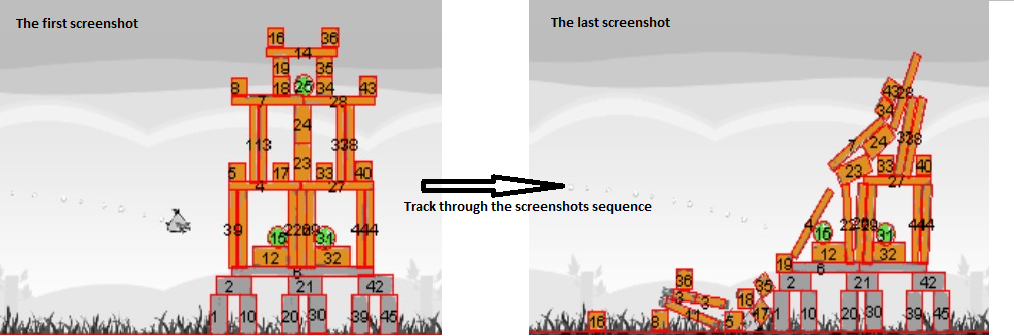
\includegraphics[scale=0.32]{TrackingBackup.png}\caption{The method tracks through the screenshots and label the matched objects with the same ID. The match between the first and last screenshots is saved as the ground truth }
\label{Tracking}
\end{figure}

To automate this process, we run an angry birds agent that always aims at an random pig on the first 21 Poached Eggs Levels \cite{abGame}. The agent starts to capture screenshots once a shot is made, and stops after 10 seconds. In each level, the agent records the screenshots of at most four shots. We removed all the samples where all the objects are stationary (the bird did not hit anything). Finally we have 62 samples.  To evaluate the accuracy of the ground truth, we run our method on 10 samples randomly picked from the 62. We get the accuracy by manually labelling the initial objects and their correspondence in the end screenshot, and compare with the matching result generated by the method. 

It turns out that the method can match most of the objects with less than 4 mismatches per sample. The method achieves real-time performance with average 3 ms per match. To illustrate the significant improvements achieved by the spatial reasoning, we compare our method with an approach  ($BASIC$) which matches objects by visual appearance and minimizing the centroid shift between initial and subsequent objects. We show the results in Table \ref{empiResults}.

\begin{table}[h!]
\caption{Results on the 10 samples(\,$QSR$: the proposed method, $BASIC$: the modified method )}\label{empiResults}
\centering
\begin{tabular}{c|c|c|c|c}
\hline
{} & \multicolumn{2}{c}{Accuracy} & \multicolumn{2}{c}{Mismatch}\\
\hline
Sample & QSR & BASIC & QSR & BASIC \\
\hline
1& 0.91 & 0.5 & 2 & 12\\
2&1.00 & 1.00 & 0 & 0\\
3&0.80 & 0.40 & 2 & 6\\
4&0.85 & 0.54 & 2 & 6\\
5&0.76 & 0.41 & 4 & 10\\
6&1.00 & 0.00 & 0 & 2\\
7&1.00 & 0.56 & 0 & 4\\
8&0.78 & 0.33 & 2 & 6 \\
9&0.71 & 0.42 & 2 & 4\\
10&1 & 0.5 & 0 & 2\\
\hline
\end{tabular}
\end{table}

\subsection{Experimental Results}

We evaluate our method on the 62 samples (12400 frames) with varying time gaps, namely 100 ms, 200 ms (the maximum delay in getting screenshot from the server used in Angry Birds AI competition), 300 ms (the time taken by requesting a screenshot plus the vision segmentation) and 1000 ms

For a particular time gap of size $T$, the method will track through every $T/50$ screenshots of the original sequence. The accuracy and mismatch is obtained by comparing against the saved ground truth. As expected, the accuracy drops down when applying larger time gaps (see Table \ref{empiResults_2}).  

\begin{table}[h!]
\caption{Results on the 80 samples with different time gaps}\label{empiResults_2}
\centering
\begin{tabular}{c|c|c|c|c}
\hline
Time gap (ms) & Average Accuracy & Average Mismatch \\
\hline
100 & 0.85 & 2.22\\
200 & 0.80 & 3.22\\
300 & 0.77 & 3.4\\
500 & 0.70 & 3.98\\
1000 & 0.68 & 4.22\\
\hline
\end{tabular}
\end{table}
\end{document}